\section{Angular}

\subsection{Allgemeines [M]}
\setauthor{Fabian Maar}
Angular ist ein Framework für Webapplikation, das auf der Programmiersprache Typescript basiert. Es ist eines der renommiertesten Frameworks zur Front-End-Entwicklung und wird als Open-Source-Software zur Verfügung gestellt. Besonders bietet sich Angular für Single-Page-Webanwendung an, da es ein komponentenbasiertes Framework ist. Das bedeutet, der Code ist wiederverwendbar und verkapselt. Komplexe Logiken werden auf ihre Grundelemente reduziert und beeinflussen sich nicht gegenseitig. 

\subsection{Dependency}
\setauthor{Litzlbauer Lorenz}
Um eine nachvollziehbare Auswahl zu treffen, muss verstanden werden, wie Angular
funktioniert. In den folgenden Unterabschnitten wird sich mit den Technologien auf die Angular aufgebaut ist, auseinandergesetzt. 

\subsubsection{RxJS}
\setauthor{Litzlbauer Lorenz}
ReactiveX ist eine Library für das Erstellen von asynchronen und Event-basierenden Programmen, dafür benutzt es  \emph{observable sequences}.
Die Library erweitert so, dass \emph{Observer-Design-Pattern} mit verschiedenen neuen Operatoren und händelt dabei "Lowlevel"-Funktionen wie Threading, Synchronisation, Thread-Sicherheit und das nicht-blockieren von I/O vergleiche \cite{ReactiveXIntro}

RxJS ist eine Implementierung von ReactiveX für die Programmiersprache Javascript. Angular verwendet RxJS für reaktive Programmierart.
\subsubsection{Webpack}
\setauthor{Litzlbauer Lorenz}
Die Hauptfunktion von Webpack ist es, viele verschiedenen Daten zu einem Paket für eine JavaScript Applikation zusammenzufassen, dabei optimiert es die Dateigröße, indem es mithilfe von einem selbst generierten \emph{dependency-graph} die Abhängigkeiten der Applikation überprüft und nur notwendige Teile für die JavaScript-Applikation der Daten nimmt. Bei der Zusammenfassung werden Sprachen, die der Webbrowser nicht Interpretieren kann wie Typescript, Sass uvm. in die für den Webbrowser verständlichen Gegenstücke gewandelt. Webpack hat aber auch viele andere Features. Vergleiche \cite{Webpack}
\setauthor{Litzlbauer Lorenz}
Angular benutzt Webpack um TypeScript in JavaScript und Sass bzw. Scss in Scss zu wandeln, um beim Bauen des Projektes alle Module in ein einziges zusammenzufassen und um die Applikation bei der Entwicklung zu \emph{Live-Reloading} zu unterstützen. Dabei wird bei einer Änderung im Code die gesamte Applikation geupdatet und neu gestartet. 

\subsection{Vorteile/Auswahlkriterien [M]}
\setauthor{Fabian Maar}
Dieses komponentenbasierte Programmieren war eines der vielen Gründe 
warum Angular die beste Option ist. Im Abschnitt 5 //TODO  wird nochmals deutlich, wie dieser Aspekt genutzt wird. Ein weiterer Grund, ist die einfache Einbindung von 
Libraries und deren Übersichtlichkeit, die durch ngModules ermöglicht werden. Die ständige Erweiterung und die Unterstützung von Third-Party-Libraries, die unter anderem für die 3D-Darstellung verwendet werden, wird ebenfalls von diesen ngModulen ermöglicht. 
Beispiele wie wir dieses ngModule aufgesetzt haben befinden sich im Abschnitt Landing-Page aufsetzen //TODO VERLINKEN. Auch aufgrund von persönlichen Erfahrungen im Unterricht und in anderen Projekten war Angular die beste Auswahlmöglichkeit.

\section{Webstorm}
\setauthor{Fabian Maar}
Webstorm ist eine Entwicklungsumgebung vom Unternehmen JetBrains, die sich auf die Programmiersprache JavaScript spezialisiert hat. Ebenfalls unterstützt es besonders Frameworks wie Angular. Das Webstorm besonders auf Angular optimiert wurde, zeigt sich durch viele Features, die das Entwickeln von Angular-Projekten erleichtern. So macht es Webstorm möglich, mit nur wenigen Mausklicks eine neue Angular-Dependency oder Komponente zu erstellen. Auch wird die Entwicklungszeit durch intelligente Code-Vervollständigung, Code-Formatierung, einfache Navigation und viele weitere hilfreiche Features deutlich verkürzt. 

\section{ThreeJs [L]}
\setauthor{Litzlbauer Lorenz}
ThreeJs ist eine JavaScript Library für die Darstellung von 3D-Grafiken im Web. Für die 3D-Darstellung nutzt ThreeJs meistens WebGL (mehr dazu im nächsten Abschnitt \hyperref[ThreeJs Dependency]{ThreeJs Dependency}), ein low-level Framework. WebGl hat eine hohe Komplexität. ThreeJs bietet eine Abstraktion, bei der es viele Sachen wie die 3D-Szene, Lichter, Schatten, Materialien, Texturen und 3D-Mathe händelt, um die 3D-Darstellungen im Web einfacher zu gestalten. In ThreeJs werden Geometrie, Objekte und Materialien verbunden, um ein 3D-Objekt zu erstellen. Dabei kann die Struktur einer Szene der Abbildung \ref{fig:tech:front:threejsstructure} ähneln. Vergleiche \cite{ThreeJsFund}

\begin{figure} [h t]
    \centering
    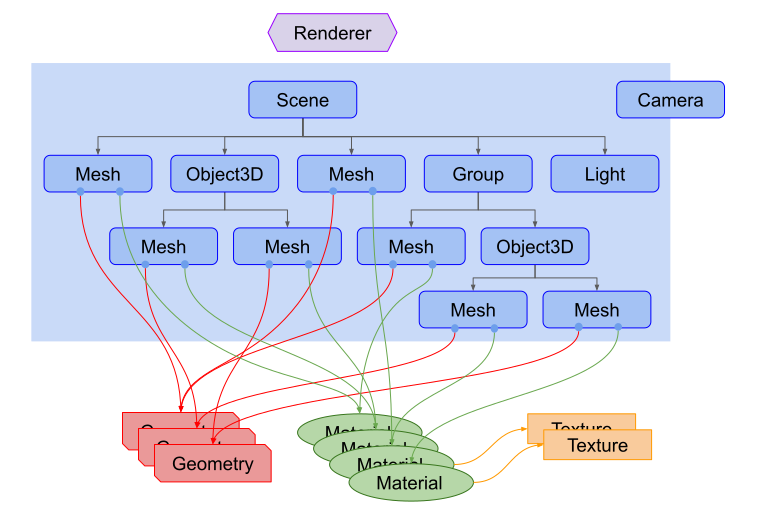
\includegraphics[scale=0.5]{pics/threejs-structure.png}
    \caption{Die Struktur von ThreeJs}
    \label{fig:tech:front:threejsstructure}
\end{figure}

\subsection{Dependency}
\label{ThreeJs Dependency}

\subsection{Vorteile/Auswahlkriterien}

